\documentclass[tikz,border=10pt]{standalone}
\usepackage{amsmath}
\usetikzlibrary{positioning,arrows.meta}

\begin{document}
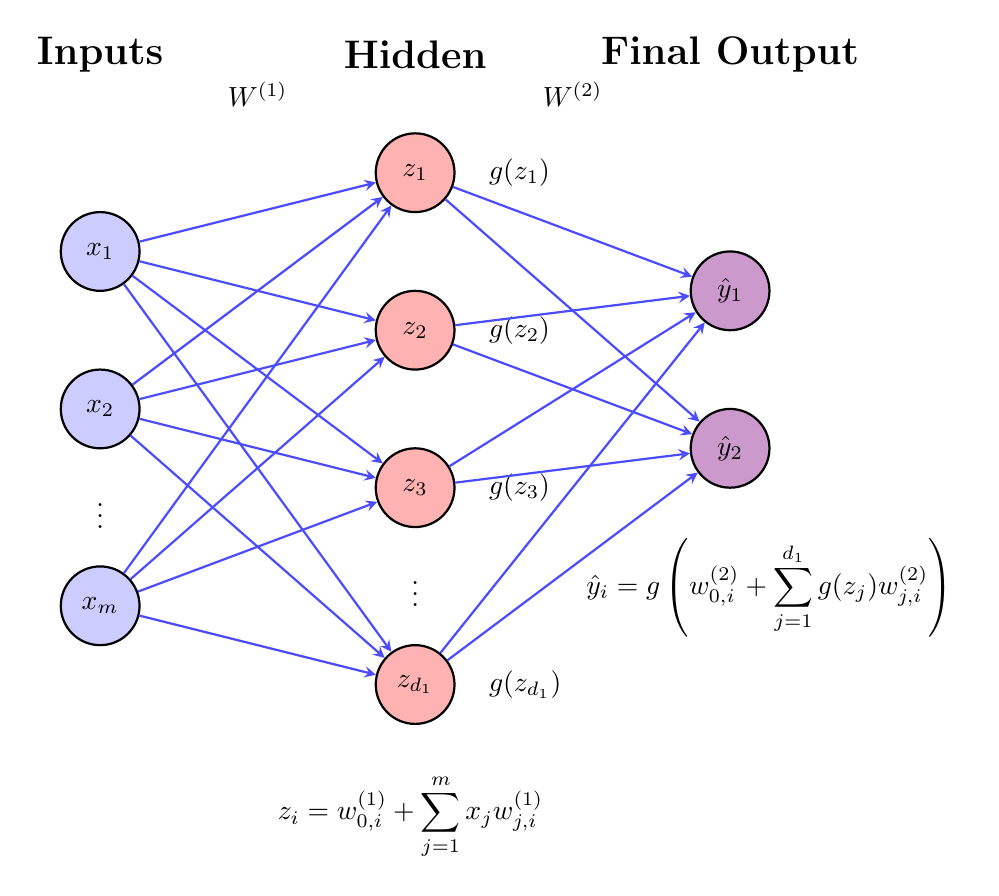
\begin{tikzpicture}[
    node distance=2cm and 3cm,
    neuron/.style={circle, draw, minimum size=1cm, thick},
    input/.style={neuron, fill=blue!20},
    hidden/.style={neuron, fill=red!30},
    output/.style={neuron, fill=violet!40},
    connection/.style={-stealth, thick, blue!70}
]

% Input layer
\node[input] (x1) at (0,2) {$x_1$};
\node[input] (x2) at (0,0) {$x_2$};
\node[input] (xm) at (0,-2.5) {$x_m$};
\node at (0,-1.25) {$\vdots$};

% Hidden layer
\node[hidden] (z1) at (4,3) {$z_1$};
\node[hidden] (z2) at (4,1) {$z_2$};
\node[hidden] (z3) at (4,-1) {$z_3$};
\node[hidden] (zd1) at (4,-3.5) {$z_{d_1}$};
\node at (4,-2.25) {$\vdots$};

% Output layer
\node[output] (y1) at (8,1.5) {$\hat{y}_1$};
\node[output] (y2) at (8,-0.5) {$\hat{y}_2$};

% Labels above layers
\node at (0,4.5) {\Large\textbf{Inputs}};
\node at (4,4.5) {\Large\textbf{Hidden}};
\node at (8,4.5) {\Large\textbf{Final Output}};

% Weight labels
\node at (2,4) {$W^{(1)}$};
\node at (6,4) {$W^{(2)}$};

% Activation function labels
\node[right=0.3cm of z1] {$g(z_1)$};
\node[right=0.3cm of z2] {$g(z_2)$};
\node[right=0.3cm of z3] {$g(z_3)$};
\node[right=0.3cm of zd1] {$g(z_{d_1})$};

% Connections from input to hidden layer
\foreach \i in {1,2,m} {
    \foreach \j in {1,2,3,d1} {
        \draw[connection] (x\i) -- (z\j);
    }
}

% Connections from hidden to output layer
\foreach \i in {1,2,3,d1} {
    \foreach \j in {1,2} {
        \draw[connection] (z\i) -- (y\j);
    }
}

% Mathematical formulas at the bottom
\node[below=5.0cm of z2, align=center] {
    $z_i = w_{0,i}^{(1)} + \displaystyle\sum_{j=1}^{m} x_j w_{j,i}^{(1)}$
};

\node[below=2.5cm of y1.south, align=center] {
    \hspace{1cm} $\hat{y}_i = g\left(w_{0,i}^{(2)} + \displaystyle\sum_{j=1}^{d_1} g(z_j) w_{j,i}^{(2)}\right)$
};

\end{tikzpicture}
\end{document}
